\documentclass[12pt,a4paper]{article}

% ============================================================
% PACKAGES
% ============================================================
\usepackage[utf8]{inputenc}
\usepackage[T1]{fontenc}
\usepackage[margin=2.5cm]{geometry}
\usepackage{array}
\usepackage{booktabs}
\usepackage{longtable}
\usepackage[table,dvipsnames]{xcolor}
\usepackage[hidelinks,colorlinks=true]{hyperref}
\usepackage{enumitem}
\usepackage{titlesec}
\usepackage{fancyhdr}
\usepackage[most]{tcolorbox}
\usepackage{tabularx}
\usepackage{setspace}
\usepackage{parskip}
\usepackage{graphicx}
\usepackage{float}

% ============================================================
% COLOR PALETTE
% ============================================================
\definecolor{accentdark}{HTML}{334155}
\definecolor{accentlight}{HTML}{DCE3EA}
\definecolor{principlebg}{HTML}{EEF1F4}
\definecolor{principleborder}{HTML}{334155}
\definecolor{grayrule}{HTML}{CCCCCC}
\definecolor{alertbg}{HTML}{F5ECEC}
\definecolor{alertborder}{HTML}{8C3A3A}
% heat-map: muted traffic light
\definecolor{heatlow}{HTML}{DCE6DD}
\definecolor{heatmed}{HTML}{EFE6D2}
\definecolor{heathigh}{HTML}{E6D2D2}

% ============================================================
% HYPERREF
% ============================================================
\hypersetup{
    linkcolor=accentdark,
    urlcolor=accentdark,
    citecolor=accentdark,
    pdftitle={GenAI-Assisted Document Redaction Governance},
    pdfauthor={Andrea Gennari}
}

% ============================================================
% SECTION STYLING
% ============================================================
\titleformat{\section}
  {\Large\bfseries\color{accentdark}}
  {\thesection}{1em}{}
  [\vspace{2pt}{\color{accentdark}\titlerule[0.7pt]}]
\titlespacing*{\section}{0pt}{24pt plus 4pt minus 2pt}{10pt plus 2pt minus 2pt}

\titleformat{\subsection}
  {\large\bfseries\color{accentdark!85!black}}
  {\thesubsection}{0.8em}{}
\titlespacing*{\subsection}{0pt}{18pt plus 3pt minus 2pt}{6pt plus 2pt minus 1pt}

% ============================================================
% HEADER / FOOTER
% ============================================================
\setlength{\headheight}{16pt}
\addtolength{\topmargin}{-4pt}
\pagestyle{fancy}
\fancyhf{}
\fancyhead[L]{\small\color{accentdark!70!black}\textit{GenAI-Assisted Document Redaction Governance}}
\fancyhead[R]{\small\color{accentdark!70!black}\textit{\nouppercase{\rightmark}}}
\fancyfoot[C]{\small\color{accentdark!70!black}\thepage}
\renewcommand{\headrulewidth}{0.4pt}
\renewcommand{\headrule}{\hbox to\headwidth{\color{accentdark!40!white}\leaders\hrule height \headrulewidth\hfill}}
\renewcommand{\footrulewidth}{0pt}

% ============================================================
% PARAGRAPH & LIST SPACING
% ============================================================
\setlength{\parskip}{6pt plus 1pt minus 1pt}
\setlength{\parindent}{0pt}

\setlist[itemize]{
  topsep=4pt, itemsep=3pt, parsep=1pt,
  leftmargin=1.8em,
  label=\textcolor{accentdark}{\textbullet}
}
\setlist[enumerate]{
  topsep=4pt, itemsep=3pt, parsep=1pt,
  leftmargin=2.2em,
  label=\textcolor{accentdark}{\arabic*.}
}

% ============================================================
% TCOLORBOX STYLES
% ============================================================
\newtcolorbox{definitionbox}[1][]{%
  enhanced, breakable, sharp corners,
  colback=white,
  colframe=accentdark,
  boxrule=0.5pt,
  coltitle=accentdark,
  colbacktitle=white,
  fonttitle=\bfseries\scshape,
  titlerule=0.4pt,
  toptitle=2pt, bottomtitle=2pt,
  left=8pt, right=8pt, top=6pt, bottom=6pt,
  title={#1},
}

\newtcolorbox{principlebox}[1][]{%
  enhanced, breakable, sharp corners,
  colback=principlebg,
  colframe=accentdark,
  boxrule=0.5pt,
  coltitle=accentdark,
  colbacktitle=principlebg,
  fonttitle=\bfseries\scshape,
  titlerule=0.4pt,
  borderline west={2pt}{0pt}{accentdark},
  toptitle=2pt, bottomtitle=2pt,
  left=10pt, right=8pt, top=6pt, bottom=6pt,
  title={#1},
}

\newtcolorbox{alertbox}[1][]{%
  enhanced, breakable, sharp corners,
  colback=white,
  colframe=alertborder,
  boxrule=0.6pt,
  coltitle=alertborder,
  colbacktitle=white,
  fonttitle=\bfseries\scshape,
  titlerule=0.4pt,
  toptitle=2pt, bottomtitle=2pt,
  left=8pt, right=8pt, top=6pt, bottom=6pt,
  title={#1},
}

\newtcolorbox{quotebox}{%
  breakable, sharp corners,
  colback=white,
  colframe=white,
  boxrule=0pt,
  borderline west={2pt}{0pt}{accentdark},
  left=10pt, right=8pt, top=4pt, bottom=4pt,
  fontupper=\itshape,
}

% ============================================================
% DOCUMENT BEGIN
% ============================================================
\begin{document}

\begin{titlepage}
    \centering
    \vspace*{3cm}

    {\color{accentdark}\rule{\textwidth}{1.5pt}}

    \vspace{1.2cm}
    {\Huge\bfseries\color{accentdark} GenAI-Assisted Document\par}
    \vspace{0.3cm}
    {\Huge\bfseries\color{accentdark} Redaction Governance\par}
    \vspace{0.8cm}
    {\Large\color{accentdark!80!black} A Governance Framework for Safe Adoption\par}
    \vspace{1.2cm}

    {\color{accentdark}\rule{0.4\textwidth}{0.8pt}}

    \vspace{2cm}
    {\large\color{accentdark!70!black} Submitted by\par}
    \vspace{0.3cm}
    {\LARGE\bfseries\color{accentdark} Andrea Gennari\par}
    \vspace{0.5cm}
    {\normalsize\color{accentdark!70!black} Business and Project Management\par}
    \vfill
    {\color{accentdark}\rule{\textwidth}{1.5pt}}
    \vspace{0.5cm}
    {\large\color{accentdark!70!black} \today\par}
\end{titlepage}

\thispagestyle{empty}
\vspace*{2cm}
\begin{tcolorbox}[
  enhanced, sharp corners,
  colback=white,
  colframe=accentdark,
  boxrule=0.5pt,
  coltitle=accentdark,
  colbacktitle=white,
  fonttitle=\bfseries\scshape,
  title=Abstract,
  titlerule=0.4pt,
  toptitle=2pt, bottomtitle=2pt,
  left=12pt, right=12pt, top=8pt, bottom=8pt,
]
This paper proposes a governance framework for the safe adoption of Generative AI-assisted document redaction tools. The central research question is: how can organizations adopt GenAI-assisted redaction through governance, human-in-the-loop controls, audit logging and risk management? The framework is organized in four pillars anchored to GDPR, the NIST AI Risk Management Framework and ISO/IEC 42001, and is illustrated against the Post Office Horizon data breach case.
\end{tcolorbox}

\newpage

\tableofcontents
\newpage

% ============================================================
% PART I — THE GOVERNANCE FRAMEWORK
% ============================================================
\begin{center}
{\color{accentdark}\rule{\textwidth}{1.2pt}}\\[6pt]
{\Huge\bfseries\color{accentdark} Part I}\\[8pt]
{\LARGE\bfseries\color{accentdark!85!black} A Governance Framework for Safe Adoption}\\[8pt]
{\color{accentdark}\rule{\textwidth}{1.2pt}}
\end{center}
\vspace{8pt}

\begin{quotebox}
\textbf{Guiding question for Part I.} How can organizations adopt GenAI-assisted document redaction safely, through governance, human-in-the-loop controls, audit logging and risk management?
\end{quotebox}

% ============================================================
\section{Framing and Foundations}
\label{sec:foundations}

\subsection{Framework Overview}

Organizations that publish documents externally need a controlled, auditable process to identify and redact sensitive content before release. GenAI can support this, but adopting it without governance adds new risks: over-reliance on automation, lost accountability, and data leakage.

This paper proposes a \textbf{governance framework} for that path, in four pillars, each addressing a distinct failure mode: Governance, Human-in-the-Loop Controls, Audit Logging, and Risk Management. Table~\ref{tab:structure} shows the structure.

\begin{table}[H]
\centering
\small
\rowcolors{2}{accentlight!30!white}{white}
\begin{tabular}{@{} p{4.8cm} p{9cm} @{}}
\toprule
\textbf{\color{accentdark}Section} & \textbf{\color{accentdark}Content} \\
\midrule
\S\ref{sec:foundations}: Foundations & Criteria for safe adoption and regulatory baseline \\
\S\ref{sec:governance}: Pillar~I & Governance, policy and accountability structure \\
\S\ref{sec:hitl}: Pillar~II & Human-in-the-loop controls and document risk classification \\
\S\ref{sec:audit}: Pillar~III & Audit logging and demonstrable compliance \\
\S\ref{sec:risk}: Pillar~IV & Risk management process and register \\
\S\ref{sec:adoption} & Adoption roadmap, KPIs and business case \\
\bottomrule
\end{tabular}
\caption{Structure of the paper.}
\label{tab:structure}
\end{table}

It is designed in full, then deployed through a limited pilot before scaling: predictive design, iterative rollout, a hybrid lifecycle \cite{falchi_slides}.

\subsection{Defining ``Safe Adoption''}
\label{sec:safe_adoption}

The framework must be verifiable. Five criteria define safe adoption; the framework is designed to satisfy all five at once.

\begin{definitionbox}[Five Criteria for Safe Adoption]
\begin{enumerate}
  \item \textbf{No unauthorized disclosure.} No personal or confidential data leaves without passing documented review and approval. (The Post Office Horizon incident is the motivating failure.)

  \item \textbf{Regulatory compliance.} Satisfies GDPR Art.~25 (protection by design) and Art.~32 (appropriate measures), and the ICO expectation of a documented pre-publication control.

  \item \textbf{Accountability and auditability.} Every document yields a record of what was done, by whom, and when, demonstrable to a regulator or court (GDPR Art.~5(2)).

  \item \textbf{Preserved human oversight.} No high-risk document is published without explicit human approval. GenAI \emph{supports}, it does not \emph{replace}, the reviewer, who is the final gate.

  \item \textbf{Sustainable adoption.} The framework is embedded: staff trained, process followed, KPIs met in the pilot. A correct framework that is bypassed reduces no risk.
\end{enumerate}
\end{definitionbox}

Each criterion has a failure condition that triggers escalation, the inverse of the criterion: any unredacted content published; any document processed outside the GDPR Art.~25/32 controls; any incomplete audit record; any high-risk release without recorded approval; KPI targets missed beyond tolerance or the process systematically bypassed. Each criterion is SMART: specific, measurable, attainable in the pilot, relevant, time-bound \cite{falchi_slides}.

\subsection{Regulatory and Standards Baseline}
\label{sec:baseline}

Three layers constrain any GenAI redaction tool: EU data-protection law, UK supervisory expectations, and international management-systems standards. Together they set the non-negotiable floor.

\noindent\textbf{GDPR: Key Articles}~\cite{gdpr}\par

\textbf{Art.~25 (by design and by default)}: protection must be built into the system \emph{before} processing, not retrofitted. Here: the review gate is part of the default publication path, not a skippable add-on.

\textbf{Art.~32 (security of processing)}: ``appropriate technical and organisational measures.'' Technical $=$ GenAI detection plus mandatory human review; organisational $=$ the policy, training, and audit log.

\textbf{Art.~5(2) (accountability)}: the controller must \emph{demonstrate} compliance. This drives Pillar~III: without a tamper-evident record of each decision, the organization cannot prove to the ICO or a court that the controls operated.

\noindent\textbf{ICO Expectations}\par

The ICO's 2025 reprimand of Post Office Limited held that publishing personal data without a documented pre-publication control breaches Art.~5(1)(f) and Art.~32 \cite{ico2025}. Its corrective requirement, a documented and auditable review process, is the origin of Pillars~II and~III, and it sets the bar: not just having a process, but proving it ran for every document.

\noindent\textbf{NIST AI RMF (1.0)}\par
The NIST AI RMF \cite{nist_ai_rmf} organises AI risk around four functions: \textbf{GOVERN} (policy, accountability, risk culture), \textbf{MAP} (context and potential harms), \textbf{MEASURE} (metrics and testing), \textbf{MANAGE} (response and monitoring). Pillar~I operationalises GOVERN; Pillar~IV covers MAP, MEASURE and MANAGE.

\noindent\textbf{ISO/IEC standards}\par
\textbf{42001:2023} \cite{iso42001} (AI management): pre-deployment risk assessment (Cl.~6), documented human oversight (A.6), data-subject impact evaluation (A.9). \textbf{27001:2022} \cite{iso27001} (information security): information classification (A.8.2), data masking (A.8.11), logging (A.8.15). The pillar that meets each clause is in Table~\ref{tab:standards}.

\noindent\textbf{Requirement Mapping}\par

Table~\ref{tab:standards} maps each requirement to its source and pillar; every row ties back to a safe-adoption criterion (Section~\ref{sec:safe_adoption}).

\begin{table}[H]
\centering
\small
\rowcolors{2}{accentlight!30!white}{white}
\begin{tabular}{@{} p{4.3cm} p{3.5cm} p{5.7cm} @{}}
\toprule
\textbf{\color{accentdark}Requirement} & \textbf{\color{accentdark}Source} & \textbf{\color{accentdark}Addressed in} \\
\midrule
Data protection by design & GDPR Art.~25 & Pillar~I (policy mandate) + Pillar~II (default review gate) \\
Appropriate security measures & GDPR Art.~32 & Pillar~I + II + III \\
Demonstrable accountability & GDPR Art.~5(2) & Pillar~III (immutable audit log) \\
Documented pre-publication control & ICO reprimand 2025 & Pillar~II (HITL review gate) \\
AI governance and risk culture & NIST AI RMF GOVERN & Pillar~I (governance structure, RACI) \\
AI risk identification & NIST AI RMF MAP & Pillar~IV (risk register) \\
AI risk measurement & NIST AI RMF MEASURE & Pillar~IV (performance metrics and KPIs) \\
AI risk treatment & NIST AI RMF MANAGE & Pillar~IV (response strategies) \\
AI human oversight & ISO/IEC 42001 A.6 & Pillar~II (mandatory human approval) \\
AI impact assessment & ISO/IEC 42001 Cl.~6 & Pillar~IV (pre-deployment risk assessment) \\
Information classification & ISO/IEC 27001 A.8.2 & Pillar~II (document risk tiers) \\
Audit evidence & ISO/IEC 27001 A.8.15 & Pillar~III (audit log) \\
\bottomrule
\end{tabular}
\caption{Regulatory and standards requirements mapped to framework pillars.}
\label{tab:standards}
\end{table}

\subsection{Framework Architecture}
\label{sec:architecture}

The framework is a \textbf{governance spine} (Pillar~I) giving authority to three operational pillars, all feeding a hybrid adoption lifecycle. One design principle governs everything that follows:

\begin{principlebox}[Architectural Principle]
\textbf{AI suggests, humans approve, the organization remains accountable.} The tool is a detection assistant, not a decision authority: every publication decision is owned by a named human and recorded in the log, and the policy, not the tool's confidence score, sets when approval is mandatory.
\end{principlebox}

\noindent\textbf{The Governance Spine}\par

Pillar~I is load-bearing: the policy mandate, the accountability hierarchy, and the RACI matrix that authorize the other three pillars, much as a project charter formally authorizes a project and names its sponsor \cite{falchi_slides} (detailed in Section~\ref{sec:governance}).

\noindent\textbf{The Three Operational Pillars}\par

\begin{itemize}
  \item \textbf{Pillar~II (Human-in-the-Loop)} classifies every document into risk tiers and routes it through the matching review gate (Section~\ref{sec:hitl}).
  \item \textbf{Pillar~III (Audit Logging)} records every action in an immutable, queryable log kept as regulatory evidence (Section~\ref{sec:audit}).
  \item \textbf{Pillar~IV (Risk Management)} keeps a living risk register, tracks residual risk and triggers escalation at thresholds (Section~\ref{sec:risk}).
\end{itemize}

\noindent\textbf{Document Flow Through the Framework}\par

The path runs from draft to publication in seven steps, linear for standard documents and gated by an approval step before the token issues for high and very-high ones. The full gated flow, with the control at each step, is Table~\ref{tab:workflow} in Section~\ref{sec:hitl}.

\noindent\textbf{Hybrid Adoption Lifecycle}\par

The framework is designed predictively (all four pillars defined before the pilot) but deployed iteratively: a controlled pilot generates KPI data and calibrates the risk-tier thresholds and review workloads before full rollout. This hybrid sequencing (Section~\ref{sec:foundations}) cuts adoption risk without losing coherence \cite{falchi_slides}.

% ============================================================
\section{Governance (Pillar I)}
\label{sec:governance}

Pillar~I is the governance spine (Section~\ref{sec:architecture}): it gives the other three pillars their authority through four artefacts: an operating model, a redaction policy, decision rights, and a RACI matrix. Without it the audit log is optional, the review gate is skippable, and the risk register has no owner.

\subsection{Operating Model and Oversight}

The framework is owned end to end by the \textbf{Data Protection Officer (DPO)}, who chairs a \textbf{Redaction Governance Board}: the oversight forum that approves the policy, sets the Pillar~II risk thresholds, reviews KPI and audit data (Section~\ref{sec:audit}), and authorizes exceptions. Five roles staff the workflow:

\begin{definitionbox}[Governance Roles]
\begin{itemize}
  \item \textbf{Document Owner}: submits the document, runs the GenAI scan, performs first-line review, and publishes against the approval token.
  \item \textbf{Legal}: advises on litigation, contractual and disclosure sensitivity; recommends on high-risk release.
  \item \textbf{DPO / Privacy}: accountable owner of the framework; chairs the Board; holds classification and high-risk approval authority; attests to audit-log integrity.
  \item \textbf{IT Security}: owns the GenAI pipeline, the vendor assessment, access controls and the log infrastructure.
  \item \textbf{Manager}: holds operational accountability for the routine flow; provides resources and owns the KPIs.
\end{itemize}
\end{definitionbox}

These parties differ in power and interest, so the framework engages them differently \cite{falchi_slides}:

\begin{itemize}
  \item \textbf{DPO, Legal} (high power, high interest): \emph{manage closely}; on the Board, with approval rights.
  \item \textbf{IT Security} (high power, lower interest): \emph{keep satisfied}; owns the controls, consulted per document.
  \item \textbf{Document owners} (lower power, high interest): \emph{keep informed} and trained.
  \item \textbf{Senior management} (high power): \emph{keep satisfied} via the Board's reporting line.
\end{itemize}

Communication splits the same way: approval decisions are \emph{pull} (recorded, retrieved on demand); policy changes and incidents are \emph{push} to every owner \cite{falchi_slides}.

\subsection{GenAI-Assisted Redaction Policy}

The policy is the artefact GDPR Art.~25 demands: it embeds data protection into the process \emph{by default}, rather than leaving it to individual diligence under time pressure.

\begin{definitionbox}[Redaction Policy at a Glance]
\begin{itemize}
  \item \textbf{Purpose}: ensure no document is shared or published externally without a documented, risk-proportionate redaction review.
  \item \textbf{Scope}: every document leaving the organization to a named external party or the public, and all staff who publish.
  \item \textbf{Core principle}: AI suggests, humans approve, the organization remains accountable (Section~\ref{sec:architecture}).
  \item \textbf{Prohibited uses}: no automatic publication at any tier; no pasting of documents into consumer GenAI tools outside the approved pipeline; no disabling of the audit log.
  \item \textbf{Vendor \& data handling}: a Data Processing Agreement (GDPR Art.~28), a contractual no-training clause, EU or approved data residency, and encryption in transit and at rest.
\end{itemize}
\end{definitionbox}

The vendor rules close a risk nothing else can: sending text to an external model is itself a disclosure. They are the control for the ``data exposure to external AI vendor'' risk (Section~\ref{sec:risk}).

\subsection{Decision Rights and Approval Gates}

Decision rights answer one question (\emph{who may authorize external release?}); the answer rises with the risk tier (Section~\ref{sec:hitl}). No tier permits automatic release: a human must record approval before a document advances. The tier-by-tier mapping of release authority and gate rule is consolidated in Table~\ref{tab:risktier} (Section~\ref{sec:hitl}).

A \textbf{gate} is a hard stop: no publication until the named authority records approval in the log (Pillar~III). The very-high tier adds \emph{dual control} so no single person can release the most sensitive material. These gates operationalize the ``preserved human oversight'' criterion (Section~\ref{sec:safe_adoption}).

\subsection{RACI Matrix}

Every activity has exactly one \textbf{Accountable} and at least one \textbf{Responsible} role, with Consulted and Informed named alongside \cite{falchi_slides}. Operational steps answer to the Manager; privacy-critical control points answer to the DPO.

\begin{table}[H]
\centering
\small
\rowcolors{2}{accentlight!30!white}{white}
\begin{tabular}{@{} >{\bfseries\color{accentdark}}p{4.4cm} *{5}{>{\centering\arraybackslash}p{1.75cm}} @{}}
\toprule
\textbf{\color{accentdark}Activity} & \textbf{\color{accentdark}Doc Owner} & \textbf{\color{accentdark}Legal} & \textbf{\color{accentdark}DPO} & \textbf{\color{accentdark}IT Sec.} & \textbf{\color{accentdark}Manager} \\
\midrule
Intake \& version check & R & I & I & C & A \\
GenAI sensitive-data scan & R & I & C & A & I \\
Risk-tier classification & R & C & A & C & I \\
Redaction proposal review & R & C & C & I & A \\
High-risk release approval & I & R & A & C & C \\
Final publication & R & I & I & C & A \\
Audit review & I & C & A & R & I \\
\bottomrule
\end{tabular}
\caption{RACI matrix for the redaction governance workflow.}
\label{tab:raci}
\end{table}

\begin{tcolorbox}[
  enhanced, sharp corners, colback=white, colframe=gray!45, boxrule=0.5pt,
  left=8pt, right=8pt, top=5pt, bottom=5pt,
]
\textbf{Legend:}\quad R\,=\,Responsible\quad A\,=\,Accountable\quad C\,=\,Consulted\quad I\,=\,Informed
\end{tcolorbox}

Two assignments carry the weight. \textbf{High-risk approval}: Accountable to the DPO, Responsible to Legal, so it is single-owned yet never decided without an independent recommendation. \textbf{Audit review}: Responsible to IT Security (who runs the log), Accountable to the DPO (who attests to it), preserving separation of duties. Every Accountable cell is a Board member.

% ============================================================
\section{Human-in-the-Loop Controls (Pillar II)}
\label{sec:hitl}

Pillar~II turns ``AI suggests, humans approve'' into procedure: it classifies every document into a risk tier, binds each tier to a level of human control, and routes it through gated review and escalation. Human attention is spent in proportion to risk.

\subsection{Document Classification and Risk Scoring}

Classification is the first control and runs on \emph{every} document. Three factors are scored; their product sets the tier.

\begin{definitionbox}[Risk Score $=$ Sensitivity $\times$ Exposure $\times$ Audience]
\begin{itemize}
  \item \textbf{Sensitivity}: the data categories present: 1~$=$ routine business; 2~$=$ personal data; 3~$=$ special-category, financial or litigation data.
  \item \textbf{Exposure}: the number of data subjects affected: 1~$=$ few; 2~$=$ tens; 3~$=$ hundreds or more.
  \item \textbf{Audience}: the reach on release: 1~$=$ internal; 2~$=$ a named external party; 3~$=$ the public web.
\end{itemize}
\end{definitionbox}

The score (1 to 27) maps to the three tiers of Section~\ref{sec:architecture}: \textbf{standard} ($\leq 4$), \textbf{high} ($6$ to $12$), \textbf{very high} ($\geq 18$). Override: any \emph{public} document (Audience~$=3$) is floored at \textbf{high}, since public release is irreversible. The Post Office document scored the maximum ($3\times3\times3=27$); Part~II shows the framework would have flagged it very high.

\subsection{Risk-Tier to Control Matrix}

The tier fixes the level of human control. Across every tier the GenAI tool only \emph{proposes}; it never publishes. What rises with risk is the seniority and number of humans who must sign off.

\begin{table}[H]
\centering
\footnotesize
\rowcolors{2}{accentlight!30!white}{white}
\begin{tabular}{@{} p{1.3cm} p{2.4cm} p{3.2cm} p{2.5cm} p{3.3cm} @{}}
\toprule
\textbf{\color{accentdark}Tier} & \textbf{\color{accentdark}GenAI role} & \textbf{\color{accentdark}Mandatory human control} & \textbf{\color{accentdark}Release authority} & \textbf{\color{accentdark}Gate rule} \\
\midrule
Standard & Proposes; flags candidates & Owner reviews every proposal and attests completeness & Document owner & Owner attests review complete; token issued on attestation \\
High & Proposes redactions & Independent reviewer (not the author) plus compliance check & DPO, on Legal's recommendation & No release until DPO approval recorded; author cannot self-approve \\
Very high & Proposes redactions & Independent review plus dual approval; no single-person release & DPO + senior management & Two recorded approvals; no single person can release \\
\bottomrule
\end{tabular}
\caption{Tier to GenAI role, human control, release authority and gate rule. No tier allows automatic release.}
\label{tab:risktier}
\end{table}

\subsection{Review and Escalation Workflow}

Table~\ref{tab:workflow} sets out the seven-step flow with, at each step, the control gate (what must hold before advancing) and the escalation branch.

\begin{table}[H]
\centering
\small
\rowcolors{2}{accentlight!30!white}{white}
\begin{tabular}{@{} c p{2.9cm} p{4.1cm} p{4.9cm} @{}}
\toprule
\textbf{\color{accentdark}\#} & \textbf{\color{accentdark}Actor (lane)} & \textbf{\color{accentdark}Action} & \textbf{\color{accentdark}Gate / escalation} \\
\midrule
1 & Document owner & Submit draft and intended audience & (none) \\
2 & System & Score and classify the tier & Public audience floors the tier at high \\
3 & GenAI tool & Propose redactions with confidence scores & Low-confidence items flagged for mandatory attention \\
4 & Reviewer & Confirm or override each proposal; attest completeness & High / very high require an \emph{independent} reviewer \\
5 & Approver & Approve the redacted version & High: DPO gate. Very high: DPO + senior (dual). A disagreement between reviewer and approver escalates to the Board \\
6 & Audit log & Lock the record; issue approval token & No token without a complete record \\
7 & Document owner & Publish against the token & Publication blocked without a valid token \\
\bottomrule
\end{tabular}
\caption{Gated review-and-escalation workflow (swimlane by actor).}
\label{tab:workflow}
\end{table}

\subsection{Reviewer Guidance and Automation Bias}

The weak point of any human-in-the-loop design is \emph{automation bias}: if reviewers rubber-stamp the tool, the gate is theatre and the over-reliance risk (Section~\ref{sec:risk}) materializes. Four choices counter it:

\begin{itemize}
  \item \textbf{Show the original, not just the result.} The reviewer sees the source document beside the proposals, so a \emph{missing} redaction is visible rather than hidden in clean-looking output.
  \item \textbf{Make confirmation an act, not a default.} The reviewer positively confirms each proposed redaction, and a ``no sensitive data'' outcome requires an explicit attestation: a recorded decision, never a silent pass.
  \item \textbf{Measure catch rate.} Blind quality samples (documents seeded with known sensitive items) test whether reviewers catch what the tool misses; the catch rate is a KPI (Section~\ref{sec:adoption}).
  \item \textbf{Gate on competence.} Only trained reviewers are provisioned, and high-risk review requires additional training, the control for the ``lack of staff training'' risk.
\end{itemize}

In PM terms, classification is probability/impact prioritization and escalation is structured decision-making \cite{falchi_slides}.

% ============================================================
\section{Audit Logging and Accountability (Pillar III)}
\label{sec:audit}

Pillar~III turns the workflow into evidence. GDPR Art.~5(2) requires the organization to \emph{demonstrate} compliance, not just achieve it, and the ICO's reprimand of Post Office Limited turned on the absence of a documented pre-publication process \cite{ico2025}. The log is the artefact that proves, for any document, that the Art.~32 controls operated.

\subsection{Purpose and Principles}

\begin{principlebox}[Three Properties of the Log]
\textbf{Complete}: every document that enters the workflow produces a record; no record, no publication token.\par
\textbf{Immutable}: entries are append-only and tamper-evident (hash-chained), so a record cannot be edited after the fact to look compliant.\par
\textbf{Traceable}: every entry binds an action to an identified actor and a timestamp, so the whole decision chain can be reconstructed.
\end{principlebox}

Completeness is enforced by the Pillar~II token gate; immutability earns a regulator's trust; traceability answers ``who decided this, and when?''

\subsection{Audit Log Schema}

Four field groups, plus the controls that protect the log itself:

\begin{definitionbox}[Audit Log Schema]
\begin{itemize}
  \item \textbf{Document identity}: document ID; type; version hash; owner; intended audience; classification tier.
  \item \textbf{Detection}: GenAI model and version; sensitive-data categories detected; per-item confidence scores; scan timestamp.
  \item \textbf{Decision}: reviewer identity; each proposal confirmed or overridden; changes made; completeness attestation; escalation flag.
  \item \textbf{Disposition}: approver identity; approval or rejection; approval timestamp; approval token ID; publication status.
\end{itemize}
\textbf{Controls on the log:} append-only (no edit or delete for any role); read access restricted to DPO and IT Security; access to the log is itself logged; retention aligned to the limitation period for related claims, then deletion (GDPR Art.~5(1)(e), storage limitation).
\end{definitionbox}

Recording the model version and per-item confidence lets an investigation separate a tool failure (item never flagged) from a reviewer failure (flagged but dismissed).

\subsection{Demonstrable Compliance}

The test of the log is whether it answers a regulator: to ``show that document~X was handled correctly,'' one query returns who scanned it, what was detected, who reviewed and changed it, who approved it, and when. Table~\ref{tab:compliance} maps log elements to requirements.

\begin{table}[H]
\centering
\small
\rowcolors{2}{accentlight!30!white}{white}
\begin{tabular}{@{} p{6.0cm} p{8.0cm} @{}}
\toprule
\textbf{\color{accentdark}Log element} & \textbf{\color{accentdark}Requirement satisfied} \\
\midrule
Complete per-document record & GDPR Art.~5(2) accountability; ICO documented-process expectation \\
Reviewer and approver identity + timestamp & Art.~32 (which control operated, and by whom); preserved-oversight criterion \\
Detected categories and redaction changes & Art.~32 (evidence the measure worked); ``no unauthorized disclosure'' criterion \\
Append-only, tamper-evident storage & Evidential integrity for the ICO or a court \\
Retention limit and restricted access & Art.~5(1)(e) storage limitation; Art.~32 confidentiality \\
\bottomrule
\end{tabular}
\caption{Audit-log elements mapped to the requirements they evidence.}
\label{tab:compliance}
\end{table}

\subsection{Audit Review Process}

The log is reviewed, not just retained: monthly, the DPO reviews a sample plus \emph{every} very-high record; quarterly, the Board reviews KPIs and exceptions. Any anomaly (missing approver, bypassed gate, incomplete record, KPI breach) is logged as an incident and escalated, closing the loop with Pillar~IV. In PM terms, the log is project documentation and configuration management: the controlled record that makes the process auditable and turns ``a control exists'' into a verifiable baseline \cite{falchi_slides}.

% ============================================================
\section{Risk Management (Pillar IV)}
\label{sec:risk}

Pillar~IV manages the risk of the tool itself. Automation removes some risk (human inconsistency, volume misses) and adds new risk (automation bias, vendor exposure, false confidence). The PMI process identifies, scores, treats, and monitors it \cite{falchi_slides}.

\subsection{Risk Management Approach}

The PMI process has six steps, and each already has a home in the framework rather than living as a separate exercise:

\begin{itemize}
  \item \textbf{Plan}: the redaction policy and this pillar's method (Pillar~I).
  \item \textbf{Identify}: the risk register below.
  \item \textbf{Qualitative analysis}: the probability/impact heat map.
  \item \textbf{Quantitative analysis}: expected monetary value for the costliest risks.
  \item \textbf{Plan responses}: one of avoid / transfer / mitigate / accept per risk, mapped to Pillars I, II and III.
  \item \textbf{Monitor \& control}: the audit review (Pillar~III) and KPIs (Section~\ref{sec:adoption}), with defined triggers.
\end{itemize}

\subsection{Risk Register}

Each risk carries an ID, category, and root cause, so responses target causes. P and I are \emph{inherent} ratings (pre-control); residuals are in Table~\ref{tab:responses}.

\begin{table}[H]
\centering
\small
\rowcolors{2}{accentlight!30!white}{white}
\begin{tabular}{@{} c p{2.2cm} p{3.8cm} p{3.8cm} c c @{}}
\toprule
\textbf{\color{accentdark}ID} & \textbf{\color{accentdark}Category} & \textbf{\color{accentdark}Risk} & \textbf{\color{accentdark}Root cause} & \textbf{\color{accentdark}P} & \textbf{\color{accentdark}I} \\
\midrule
R1 & Detection & Sensitive data not detected (false negative) & Model limits; novel data formats & M & H \\
R2 & Process & Wrong document version published & No version control; manual handling & M & H \\
R3 & Human factor & Over-reliance on AI (automation bias) & Reviewer defers to the tool & M & H \\
R4 & Compliance & Cannot demonstrate compliance & No persistent record of decisions & M & H \\
R5 & Vendor / data & Document text exposed to external AI vendor & Text sent off-premise for inference & M & H \\
R6 & Quality & Excess false positives erode trust and throughput & Conservative model tuning & H & M \\
R7 & Organizational & Staff untrained; process bypassed & Rushed rollout & M & M \\
R8 & Governance & Unclear accountability for release & No defined decision rights & M & H \\
\bottomrule
\end{tabular}
\caption{Risk register (inherent probability P and impact I, before controls).}
\label{tab:riskregister}
\end{table}

\subsection{Qualitative and Quantitative Analysis}

The probability/impact grid \cite{falchi_slides} shows the profile (Table~\ref{tab:heatmap}). The cluster in the medium-probability / high-impact cell justifies a control-heavy framework: these risks are neither rare nor mild.

\begin{table}[H]
\centering
\small
\rowcolors{2}{white}{white}
\begin{tabular}{@{} c >{\centering\arraybackslash}p{2.3cm} >{\centering\arraybackslash}p{2.3cm} >{\centering\arraybackslash}p{3.6cm} @{}}
\toprule
 & \multicolumn{3}{c}{\textbf{\color{accentdark}Impact} $\rightarrow$} \\
\textbf{\color{accentdark}Probability $\downarrow$} & \textbf{Low} & \textbf{Medium} & \textbf{High} \\
\midrule
\textbf{High}   & \cellcolor{heatmed} & \cellcolor{heathigh} R6 & \cellcolor{heathigh} \\
\textbf{Medium} & \cellcolor{heatlow} & \cellcolor{heatmed} R7 & \cellcolor{heathigh} R1, R2, R3, R4, R5, R8 \\
\textbf{Low}    & \cellcolor{heatlow} & \cellcolor{heatlow} & \cellcolor{heatmed} \\
\bottomrule
\end{tabular}
\caption{Probability/impact heat map of the inherent risk register.}
\label{tab:heatmap}
\end{table}

The costliest risks are weighed by \textbf{expected monetary value} (EMV $=$ probability $\times$ impact) \cite{falchi_slides}: a control pays off when the expected loss it removes exceeds its cost. Two caveats: EMV is an average and hides the tail (the flaw of averages), so the very-high tier uses dual control rather than a cost-benefit test \cite{falchi_slides}; and these figures are illustrative, the case-calibrated EMV being deferred to the Part~II counterfactual (Section~\ref{sec:counterfactual}).

\subsection{Risk Responses and Residual Risk}

Each risk takes one of the four PMI strategies (avoid, transfer, mitigate, accept), delivered by a control in another pillar \cite{falchi_slides}: the framework is the response plan for its own register.

\begin{table}[H]
\centering
\small
\rowcolors{2}{accentlight!30!white}{white}
\begin{tabular}{@{} c p{2.4cm} p{8.2cm} >{\centering\arraybackslash}p{1.9cm} @{}}
\toprule
\textbf{\color{accentdark}ID} & \textbf{\color{accentdark}Strategy} & \textbf{\color{accentdark}Response (control $\rightarrow$ pillar)} & \textbf{\color{accentdark}Residual} \\
\midrule
R1 & Mitigate & Mandatory review of all proposals; independent review for high risk; catch-rate KPI ($\rightarrow$ II) & Low/Med \\
R2 & Mitigate & Version hash and token-gated publication ($\rightarrow$ II/III) & Low \\
R3 & Mitigate & Confirm-each-item review, original shown, blind samples, training ($\rightarrow$ II) & Low/Med \\
R4 & Mitigate & Immutable, complete audit log ($\rightarrow$ III) & Low \\
R5 & Transfer + mitigate & DPA and no-training clause shift liability; EU residency limits exposure ($\rightarrow$ I) & Low/Med \\
R6 & Accept (reduce) & Reviewer adjusts proposals; thresholds tuned in the pilot; residual false positives accepted as the cost of safety ($\rightarrow$ II) & Med \\
R7 & Avoid + mitigate & No provisioning without training; gated rollout ($\rightarrow$ I) & Low \\
R8 & Mitigate & RACI, decision rights and approval gates ($\rightarrow$ I) & Low \\
\bottomrule
\end{tabular}
\caption{Risk responses mapped to controls, with residual risk.}
\label{tab:responses}
\end{table}

All four strategies appear: most risks are \emph{mitigated}; vendor liability is partly \emph{transferred} by contract (R5); untrained-staff exposure is \emph{avoided} (R7); irreducible false positives are \emph{accepted} (R6). Residual risk is monitored via the audit review and KPIs, with \textbf{triggers} (catch rate below target, or any released-without-approval event) escalating to the Board and a contingency reserve for incidents \cite{falchi_slides}. The claim is not zero risk but controlled risk: every inherent risk moved out of the red cell of Table~\ref{tab:heatmap} and kept there.

% ============================================================
\section{Adoption, Measurement and Business Case}
\label{sec:adoption}

Criterion~5 (Section~\ref{sec:safe_adoption}) makes embedded adoption part of safe adoption, not an afterthought. This section makes it operational: a phased roadmap with go/no-go gates, the KPIs that prove the controls run, a maturity model to position progress, and the business case that justifies the spend.

\subsection{Adoption Roadmap}

Rollout follows the hybrid lifecycle of Section~\ref{sec:architecture} \cite{falchi_slides}: four phases, each closed by a \textbf{gate}, where the next phase does not start until the exit criterion is met.

\begin{table}[H]
\centering
\small
\rowcolors{2}{accentlight!30!white}{white}
\begin{tabular}{@{} p{2.0cm} p{4.7cm} p{3.4cm} p{3.4cm} @{}}
\toprule
\textbf{\color{accentdark}Phase} & \textbf{\color{accentdark}Key activities} & \textbf{\color{accentdark}Deliverable} & \textbf{\color{accentdark}Gate (go/no-go)} \\
\midrule
1. Assess & Map document flows; baseline current risk; vendor and DPA due diligence (Pillar~I) & Risk baseline; approved vendor & DPA signed; Board mandate \\
2. Design & Configure tiers and thresholds; build the log; write policy and RACI; train reviewers & Configured pipeline; trained reviewers & Policy approved; reviewers certified \\
3. Pilot & Run a bounded document set live; collect KPI data; calibrate thresholds & KPI dataset; tuned thresholds & KPI targets met; zero leakage \\
4. Scale & Extend to all publishing units; embed audit review and reporting & Org-wide rollout; steady-state KPIs & Adoption $>70\%$; sustained KPIs \\
\bottomrule
\end{tabular}
\caption{Phased adoption roadmap with exit gates.}
\label{tab:roadmap}
\end{table}

\noindent\textbf{Work breakdown and schedule.}\par
The Design phase decomposes into four work packages \cite{falchi_slides}: (WP1) vendor contracting and DPA; (WP2) pipeline integration and log infrastructure; (WP3) policy, RACI and decision rights; (WP4) reviewer training and certification. WP1 is the longest-lead item and gates WP2, so the \textbf{critical path} runs WP1~$\to$~WP2~$\to$~Pilot. Durations on the uncertain packages (integration, training) are estimated three-point (PERT: optimistic, most likely, pessimistic) to size a realistic schedule and a time buffer ahead of the pilot gate \cite{falchi_slides}.

\subsection{KPIs and Control Effectiveness}

KPIs answer one question: do the controls actually operate? They split into \textbf{leading} indicators (process health, observed continuously, allowing correction before harm) and \textbf{lagging} indicators (outcomes, confirming the framework worked). Each ties to a safe-adoption criterion and feeds the Pillar~IV triggers (Section~\ref{sec:risk}).

\begin{table}[H]
\centering
\small
\rowcolors{2}{accentlight!30!white}{white}
\begin{tabular}{@{} p{3.5cm} c p{5.0cm} >{\centering\arraybackslash}p{2.6cm} @{}}
\toprule
\textbf{\color{accentdark}KPI} & \textbf{\color{accentdark}Type} & \textbf{\color{accentdark}Formula} & \textbf{\color{accentdark}Target} \\
\midrule
Pre-publication scan rate & Lead & Documents scanned / documents published & 100\% \\
Audit completeness & Lead & Documents with a complete log / total processed & 100\% \\
High-risk approval rate & Lead & High-risk docs with recorded DPO approval / total high-risk & 100\% \\
Reviewer catch rate & Lead & Seeded items caught / seeded items planted & $\geq 95\%$ \\
Average review time & Lead & Mean time from upload to approval & $<24$h \\
User adoption rate & Lead & Active users / target users & $>70\%$ \\
False-negative rate & Lag & Sensitive items missed / total sensitive items & $<5\%$ pilot \\
Wrong-version incidents & Lag & Wrong document versions published & 0 \\
Data-leakage incidents & Lag & Confirmed leakage events & 0 \\
\bottomrule
\end{tabular}
\caption{KPIs, split into leading (process) and lagging (outcome) indicators.}
\label{tab:kpis}
\end{table}

\textbf{Control effectiveness} is read from the pairing: a leading KPI on target while a lagging KPI breaches signals a control gap, not a staffing one. The catch rate (blind seeded samples, Section~\ref{sec:hitl}) is the direct test of automation bias; a breach on any lagging indicator is a trigger that escalates to the Board with the residual risk it exposes (Section~\ref{sec:risk}).

\subsection{Maturity Model}

A five-level model positions where an organization sits and what the pilot must move. The framework targets Level~4 by end of pilot, Level~5 at steady state.

\begin{table}[H]
\centering
\small
\rowcolors{2}{accentlight!30!white}{white}
\begin{tabular}{@{} c p{2.6cm} p{8.8cm} @{}}
\toprule
\textbf{\color{accentdark}L} & \textbf{\color{accentdark}Stage} & \textbf{\color{accentdark}Characteristic} \\
\midrule
1 & Ad hoc & Redaction is manual and discretionary; no policy, no record (the Post Office baseline) \\
2 & Defined & Policy, tiers and RACI exist on paper; application is inconsistent \\
3 & Managed & HITL gates and audit log operate for every document \\
4 & Measured & KPIs are collected and drive threshold and workload calibration \\
5 & Optimized & Metrics feed continuous improvement; controls self-correct on triggers \\
\bottomrule
\end{tabular}
\caption{Redaction-governance maturity model.}
\label{tab:maturity}
\end{table}

\subsection{Business Case}

This is the project \textbf{business case}, reframed: \textbf{risk-driven, not cost-saving driven}. Direct annual cost may rise, while the value is the expected loss avoided, so the justification is a risk-adjusted return on investment rather than a cheaper-processing saving \cite{falchi_slides}. Assume 200 externally published documents per year.

\begin{table}[H]
\centering
\small
\rowcolors{2}{accentlight!30!white}{white}
\begin{tabular}{@{} p{6.0cm} >{\raggedleft\arraybackslash}p{3.4cm} >{\raggedleft\arraybackslash}p{3.4cm} @{}}
\toprule
\textbf{\color{accentdark}Item} & \textbf{\color{accentdark}Manual} & \textbf{\color{accentdark}GenAI-assisted} \\
\midrule
Average review time & 45 min & 20 min \\
Total review hours (at EUR 35/h) & 150 & 66.7 \\
Human review cost & EUR 5,250 & EUR 2,334 \\
Software / API cost & EUR 0 & EUR 10,000 \\
\textbf{Total annual cost} & \textbf{EUR 5,250} & \textbf{EUR 12,334} \\
\bottomrule
\end{tabular}
\caption{Illustrative direct-cost comparison (pilot scale).}
\label{tab:businesscase}
\end{table}

The framework costs about EUR 7,000 more per year in direct terms. The return is on the risk side: a single publication of unredacted personal data exposes regulatory fines, compensation and reputational loss far above this figure. Treating the framework as a risk-reduction investment, it pays off when the expected loss it removes (probability of a breach $\times$ its impact) exceeds the incremental cost: the EMV logic of Section~\ref{sec:risk}. The case-calibrated figures, anchored to the Post Office impact, are computed in the Part~II counterfactual (Section~\ref{sec:counterfactual}).

\begin{principlebox}[Bottom line]
The direct cost is the premium; the avoided expected loss is the cover. The framework is justified not by cheaper review but by the breach it prevents.
\end{principlebox}

% ============================================================
\section{Synthesis: Answering the Guiding Question}
\label{sec:synthesis}

\subsection{How the Framework Achieves Safe Adoption}

Part~I asked how an organization can adopt GenAI-assisted redaction safely (Section~\ref{sec:foundations}). The answer is structural: the four pillars are engineered so that the five criteria of Section~\ref{sec:safe_adoption} hold \emph{together}, not one at a time. Table~\ref{tab:answer} traces each criterion to the mechanism that delivers it and the evidence that shows it operating.

\begin{table}[H]
\centering
\small
\rowcolors{2}{accentlight!30!white}{white}
\begin{tabular}{@{} p{3.4cm} p{7.2cm} p{3.2cm} @{}}
\toprule
\textbf{\color{accentdark}Criterion} & \textbf{\color{accentdark}How the framework satisfies it} & \textbf{\color{accentdark}Evidence} \\
\midrule
No unauthorized disclosure & Mandatory review gate on every tier; no automatic release at any tier & \S\ref{sec:hitl}, Tab.~\ref{tab:risktier} \\
Regulatory compliance (GDPR Art.~25/32) & Policy by default plus technical and organisational measures mapped to each clause & \S\ref{sec:baseline}, Tab.~\ref{tab:standards} \\
Accountability and auditability & Complete, immutable, traceable per-document log & \S\ref{sec:audit}, Tab.~\ref{tab:compliance} \\
Preserved human oversight & Named approver per tier; dual control at very high; no single-person release & \S\ref{sec:governance}, Tab.~\ref{tab:risktier} \\
Sustainable adoption & Gated roadmap, leading and lagging KPIs, and a maturity target & \S\ref{sec:adoption}, Tab.~\ref{tab:roadmap},~\ref{tab:kpis} \\
\bottomrule
\end{tabular}
\caption{The five safe-adoption criteria mapped to the mechanism that delivers each and the evidence it operated.}
\label{tab:answer}
\end{table}

No criterion depends on goodwill or on a single control: each is carried by a named pillar and evidenced in the log, and the failure condition of each (Section~\ref{sec:safe_adoption}) is itself a monitored trigger (Section~\ref{sec:risk}). The framework is therefore a coherent path to safe adoption, not a checklist, and that is the answer to the guiding question.

\subsection{Limitations and Assumptions}

The framework reduces risk; it does not eliminate it, and it rests on assumptions that must hold for the controls to work.

\begin{definitionbox}[]
\textbf{Assumptions.}
\begin{itemize}
  \item \textbf{The GenAI tool is a competent first pass.} The design is tool-agnostic, but a weak detector raises reviewer workload rather than breaking the controls, and a strong one lowers it.
  \item \textbf{Reviewers engage genuinely.} Automation bias is mitigated (Section~\ref{sec:hitl}), not abolished; the controls assume the trained reviewer actually looks.
  \item \textbf{The vendor honours the agreement.} The Data Processing Agreement and no-training clause make R5 a transferred risk, reduced by contract, not removed.
  \item \textbf{Governance is resourced.} The Board, training and audit review carry a standing cost; criterion~5 fails if it is not paid.
\end{itemize}
\textbf{Limits.}
\begin{itemize}
  \item \textbf{Not zero risk.} Residual false negatives remain (Table~\ref{tab:responses}); the claim is controlled risk, not eliminated risk.
  \item \textbf{Designed, not yet validated.} The KPI targets are set, not demonstrated, and the cost figures are illustrative; a pilot is what would confirm them.
  \item \textbf{Bounded scope.} This is a single-organization publication workflow, not a full software architecture, a live deployment, or legal advice.
\end{itemize}
\end{definitionbox}

These are the boundary of the claim, not loose ends: the framework is an internally coherent, standards-anchored design whose effectiveness is argued here and would be measured in a pilot.



% ============================================================
% PART II — THE POST OFFICE HORIZON CASE
% ============================================================
\clearpage
\begin{center}
{\color{accentdark}\rule{\textwidth}{1.2pt}}\\[6pt]
{\Huge\bfseries\color{accentdark} Part II}\\[8pt]
{\LARGE\bfseries\color{accentdark!85!black} The Post Office Horizon Case}\\[8pt]
{\color{accentdark}\rule{\textwidth}{1.2pt}}
\end{center}
\vspace{8pt}

\begin{quotebox}
\textbf{Guiding question for Part II.} How could a GenAI-assisted governance framework have reduced the privacy and data leakage risks in the Post Office Horizon document publication case?
\end{quotebox}

% ============================================================
\section{Case Analysis: Root Causes and Governance Gaps}
\label{sec:case_analysis}

In 2024, Post Office Limited published an unredacted legal settlement document on its public website. The file carried the names and addresses of hundreds of claimants in the Horizon group litigation, and it stayed publicly reachable until it was noticed and removed \cite{guardian2024}. In 2025 the Information Commissioner's Office issued a reprimand, finding that the organization had not put in place appropriate technical and organisational measures, the standard required by GDPR Art.~32 \cite{ico2025}.

Read as a project-management failure rather than a typing slip, the breach is instructive: a single routine action (uploading a file) produced irreversible public disclosure because nothing stood between that action and the public web. The proximate cause was a wrong-file upload; the root cause was the absence of a governance layer. A short root-cause drill makes the gap explicit.

\begin{definitionbox}[Root-Cause Drill (Five Whys)]
\begin{enumerate}
  \item \textbf{Why was personal data exposed?} An unredacted version of the document was published.
  \item \textbf{Why was an unredacted version published?} The wrong file was uploaded and nothing checked it before release.
  \item \textbf{Why did nothing check it?} There was no mandatory pre-publication redaction review.
  \item \textbf{Why was there no review?} Publication carried no sensitivity classification and no approval gate.
  \item \textbf{Why was there no gate?} No role was accountable for redaction governance.
\end{enumerate}
\textbf{Root cause:} no governance layer (classification, mandatory review, approval gate, audit) sat between an individual's action and irreversible public disclosure.
\end{definitionbox}

Each ``why'' is a control the framework supplies. Table~\ref{tab:rootcause} maps the observed failures to the governance gap behind each one and to the pillar that closes it. The case is, in effect, a live realization of four risks already in the Part~I register (Table~\ref{tab:riskregister}): R2 (wrong version), R4 (cannot demonstrate compliance), R8 (unclear accountability), and an uncontrolled R1 (sensitive data never detected, because it was never scanned).

\begin{table}[H]
\centering
\small
\rowcolors{2}{accentlight!30!white}{white}
\begin{tabular}{@{} p{4.4cm} p{5.4cm} p{3.8cm} @{}}
\toprule
\textbf{\color{accentdark}What happened} & \textbf{\color{accentdark}Governance gap (root cause)} & \textbf{\color{accentdark}Missing control} \\
\midrule
Unredacted version published & No mandatory pre-publication redaction review & Pillar~II review gate \\
Wrong file version uploaded & No version control or pre-publication check & Pillar~II classification; Pillar~III token \\
Top-sensitivity document treated as routine & No document classification or risk scoring & Pillar~II risk tiers \\
Released by one person, no sign-off & No decision rights or approval gate for high-risk release & Pillar~I decision rights; Pillar~II gate \\
Could not show a controlled process & No audit trail of who did what, and when & Pillar~III audit log \\
No owner answerable for the outcome & Accountability never assigned & Pillar~I RACI and governance spine \\
\bottomrule
\end{tabular}
\caption{Post Office Horizon document breach: observed failures, root causes and the missing controls.}
\label{tab:rootcause}
\end{table}

The pattern is consistent: every gap is organizational, not technical. No new software was required to prevent this breach, only a governed process. That is the lesson the framework operationalizes \cite{falchi_slides}.

% ============================================================
\section{Applying the Framework to the Case}
\label{sec:apply_framework}

This section runs the same document through the framework, pillar by pillar, and marks the point at which each control would have stopped the breach. The input is a litigation settlement holding the personal data of hundreds of claimants, intended for the public web: the highest-stakes case the framework is designed for.

\subsection{Governance Controls (Pillar I)}

The document falls squarely inside the redaction policy's scope (an external, public release of personal data), so the process is not optional. Decision rights place a public release of litigation data in the very-high tier, where authority sits with the DPO plus senior management under dual control (Section~\ref{sec:governance}): no single employee may release it. The RACI matrix (Table~\ref{tab:raci}) names an Accountable owner for the release, so ``upload'' can no longer be the final act of one person. The gap behind R8 closes here: the decision acquires an owner and a gate.

\subsection{Human-in-the-Loop Controls (Pillar II)}

Classification is decisive. Scoring the document on the Section~\ref{sec:hitl} scale gives Sensitivity~$3$ (litigation and special-category data) $\times$ Exposure~$3$ (hundreds of subjects) $\times$ Audience~$3$ (public web) $=27$, the maximum, and the public-audience override would floor it at high even if the score were lower. That tier mandates independent review plus dual approval, with no automatic release (Table~\ref{tab:risktier}). Because the reviewer sees the source document beside the proposals and must positively clear it (Section~\ref{sec:hitl}), an unredacted file is not a clean-looking pass: the exposed names and addresses are exactly what the reviewer is required to catch. The wrong version cannot reach the publication path, because publication is blocked without an approval token (step~7 of Table~\ref{tab:workflow}).

\subsection{Audit Logging (Pillar III)}

Every step leaves a record: who classified the document, who reviewed it, what was changed, who approved it, the version hash and the timestamps (Section~\ref{sec:audit}). Publication is impossible without an approval token bound to a complete log entry, which forecloses the wrong-version upload at the technical level. Crucially, this is the precise gap the ICO penalized: instead of being unable to show a controlled process, the organization could answer the regulator with the full decision trail for the document, satisfying the accountability duty of GDPR Art.~5(2). R4 closes here.

\subsection{Risk Management (Pillar IV)}

The case is a materialized draw from the register (Section~\ref{sec:risk}): R2, R4 and R8 occurring together, with R1 left uncontrolled. The framework's responses target each one directly: version hash and token-gated publication (R2), the immutable log (R4), RACI and decision rights (R8), and mandatory classified review (R1). In monitoring terms, the ``released-without-approval'' trigger would have fired before disclosure, and the wrong-version-incident KPI (target~$0$, Table~\ref{tab:kpis}) would have flagged the event. The residual risk is a reviewer clearing a genuinely mislabelled file despite dual control: small, and itself surfaced by the audit review.

% ============================================================
\section{Counterfactual Analysis}
\label{sec:counterfactual}

Section~\ref{sec:apply_framework} shows the framework would have blocked the breach qualitatively. This section asks the quantitative question a manager would: what is the expected annual loss with and without the framework, and does the difference justify the cost? It is the case-calibrated version of the expected-monetary-value sketch deferred from Sections~\ref{sec:risk} and~\ref{sec:adoption} \cite{falchi_slides}.

\noindent\textbf{Modelling the decision.}\par
The publication step is a decision node with two branches, control on or control off, each leading to a chance node where a breach either occurs or does not. Folding the tree back on expected value needs two inputs: the probability of a publication-stage breach per year and its impact. Both are illustrative, chosen consistently with the Part~I figures; what matters is the structure and the order of magnitude, not precision (Section~\ref{sec:synthesis}).

\noindent\textbf{Impact.}\par
A serious public disclosure of special-category data for hundreds of subjects carries regulatory exposure (a reprimand in this case, with fines available in principle), remediation and notification cost, possible compensation, and reputational damage. Aggregated, an illustrative EUR 500,000 per event is conservative against the GDPR maximum.

\noindent\textbf{Probability.}\par
For an organization publishing roughly 200 sensitive documents a year with no pre-publication gate, an annual probability of one serious slip on the order of 20\% is plausible, and the Post Office outcome shows the event is far from hypothetical. The framework's mandatory classification, dual-approval gate and token reduce this to a residual of about 2\% (reviewer error despite the controls).

\begin{table}[H]
\centering
\small
\rowcolors{2}{accentlight!30!white}{white}
\begin{tabular}{@{} p{5.6cm} >{\centering\arraybackslash}p{2.6cm} >{\raggedleft\arraybackslash}p{2.4cm} >{\raggedleft\arraybackslash}p{2.6cm} @{}}
\toprule
\textbf{\color{accentdark}Scenario} & \textbf{\color{accentdark}Breach prob./yr} & \textbf{\color{accentdark}Impact} & \textbf{\color{accentdark}EMV (loss/yr)} \\
\midrule
Without framework (status quo) & 20\% & EUR 500,000 & EUR 100,000 \\
With framework & 2\% & EUR 500,000 & EUR 10,000 \\
\textbf{Expected loss avoided} & & & \textbf{EUR 90,000} \\
Less incremental cost (Table~\ref{tab:businesscase}) & & & (EUR 7,000) \\
\textbf{Net expected annual benefit} & & & \textbf{EUR 83,000} \\
\bottomrule
\end{tabular}
\caption{Expected-monetary-value counterfactual: expected annual loss with and without the framework (illustrative figures).}
\label{tab:emv}
\end{table}

On expected value, the framework returns about EUR 83,000 a year against a roughly EUR 7,000 incremental cost: a risk-adjusted payback many times over, and the deferred answer to the Part~I business case (Section~\ref{sec:adoption}).

\noindent\textbf{Why the average understates the case.}\par
EMV is a mean, and a mean hides the tail, the flaw of averages \cite{falchi_slides}. The danger here is not a steady drip of EUR 100,000 a year; it is the single catastrophic disclosure, which is exactly the event that occurred. A risk that is low-frequency but irreversible is not adequately governed by a cost-benefit average, which is why the very-high tier uses dual control rather than an EMV test (Section~\ref{sec:risk}): the framework is justified not only because expected value is positive, but because the tail outcome is one the organization cannot accept. The Post Office case is that tail outcome made real.

% ============================================================
\section{Synthesis: Lessons from the Case}
\label{sec:lessons}

Read as a lessons-learned review \cite{falchi_slides}, four lessons generalize beyond this case:

\begin{itemize}
  \item \textbf{Redaction is a governance problem.} The failure was the absence of decision rights, a gate and a record, not the absence of a better tool (Section~\ref{sec:case_analysis}).
  \item \textbf{The gate matters more than the model.} Even without GenAI, a mandatory classified review with approval and logging would have prevented the breach; GenAI lowers the cost of doing this at scale, it does not replace it.
  \item \textbf{Accountability must be assigned before the incident.} A named Accountable owner and dual control for the top tier remove the single point of failure the case exposed.
  \item \textbf{Auditability is what proves the process ran.} The ICO penalized the inability to demonstrate control; an immutable log turns ``we have a process'' into evidence (GDPR Art.~5(2)).
\end{itemize}

\newpage
% ============================================================
\section{Prototype Walkthrough}
\label{sec:prototype}

To show the framework is operational and not only conceptual, a small runnable prototype implements the Pillar~II and Pillar~III pipeline end to end. It takes a PDF in and produces a redacted PDF plus an audit record. It uses the Python standard library and one PDF library (PyMuPDF); it runs in about one second, with no model download, so it can be executed live. In PM terms it is a proof of concept: the verification-and-validation step that moves the predictive design toward a validated deliverable before the pilot of Section~\ref{sec:adoption} \cite{falchi_slides}.

\subsection{What it does}

\begin{enumerate}
  \item \textbf{Detect} (Pillar~II, the tool proposes): pattern matchers flag emails, phone numbers, postcodes, dates of birth, names, and financial identifiers (IBAN, sort code, account number, National Insurance number, monetary amounts). Each category carries a sensitivity weight (1 routine, 2 personal, 3 financial or special).
  \item \textbf{Score} (Pillar~II): the tool computes Risk $=$ Sensitivity $\times$ Exposure $\times$ Audience and maps it to a tier, applying the public-release floor of Section~\ref{sec:hitl}.
  \item \textbf{Redact}: it performs a \emph{true} redaction. The underlying text is deleted from the file and a black bar is drawn over its box, so the sensitive bytes are gone, not merely covered.
  \item \textbf{Audit} (Pillar~III): it writes a hash-chained record with the four field groups of Section~\ref{sec:audit} (identity, detection, decision, disposition). Publication status stays \texttt{BLOCKED} until a human clears the review gate.
  \item \textbf{Verify}: it re-opens the output, re-extracts the text, and confirms no flagged item is still present, the byte-level check the Post Office process never performed.
\end{enumerate}

\subsection{How to run}

\begin{definitionbox}[Commands]
\ttfamily\small
python redact\_pdf.py build\\
python redact\_pdf.py redact sample\_incident\_report.pdf
\end{definitionbox}

On the seeded sample (a draft memo flagged for public release, naming two sub-postmasters with their bank and identity data) the run reports:

\begin{definitionbox}[Run report (abridged)]
\ttfamily\scriptsize
Items detected~~~~: 13 (EMAIL, IBAN, MONEY, NI\_NUMBER, PERSON, ...)\\
RISK~(Pillar II)~~: 3 x 2 x 3 = 18~~->~~tier: VERY HIGH\\
Human control~~~~~: Independent review plus dual approval\\
Byte-level check~~: CLEAN, no sensitive text remains in the file\\
Audit (Pillar III): hash-chained record written, publication BLOCKED
\end{definitionbox}

The maximum-adjacent score (18, very high) routes the document to dual approval, exactly the control the case lacked. Figure~\ref{fig:redacted} shows the redacted output.

\begin{figure}[H]
\centering
\fbox{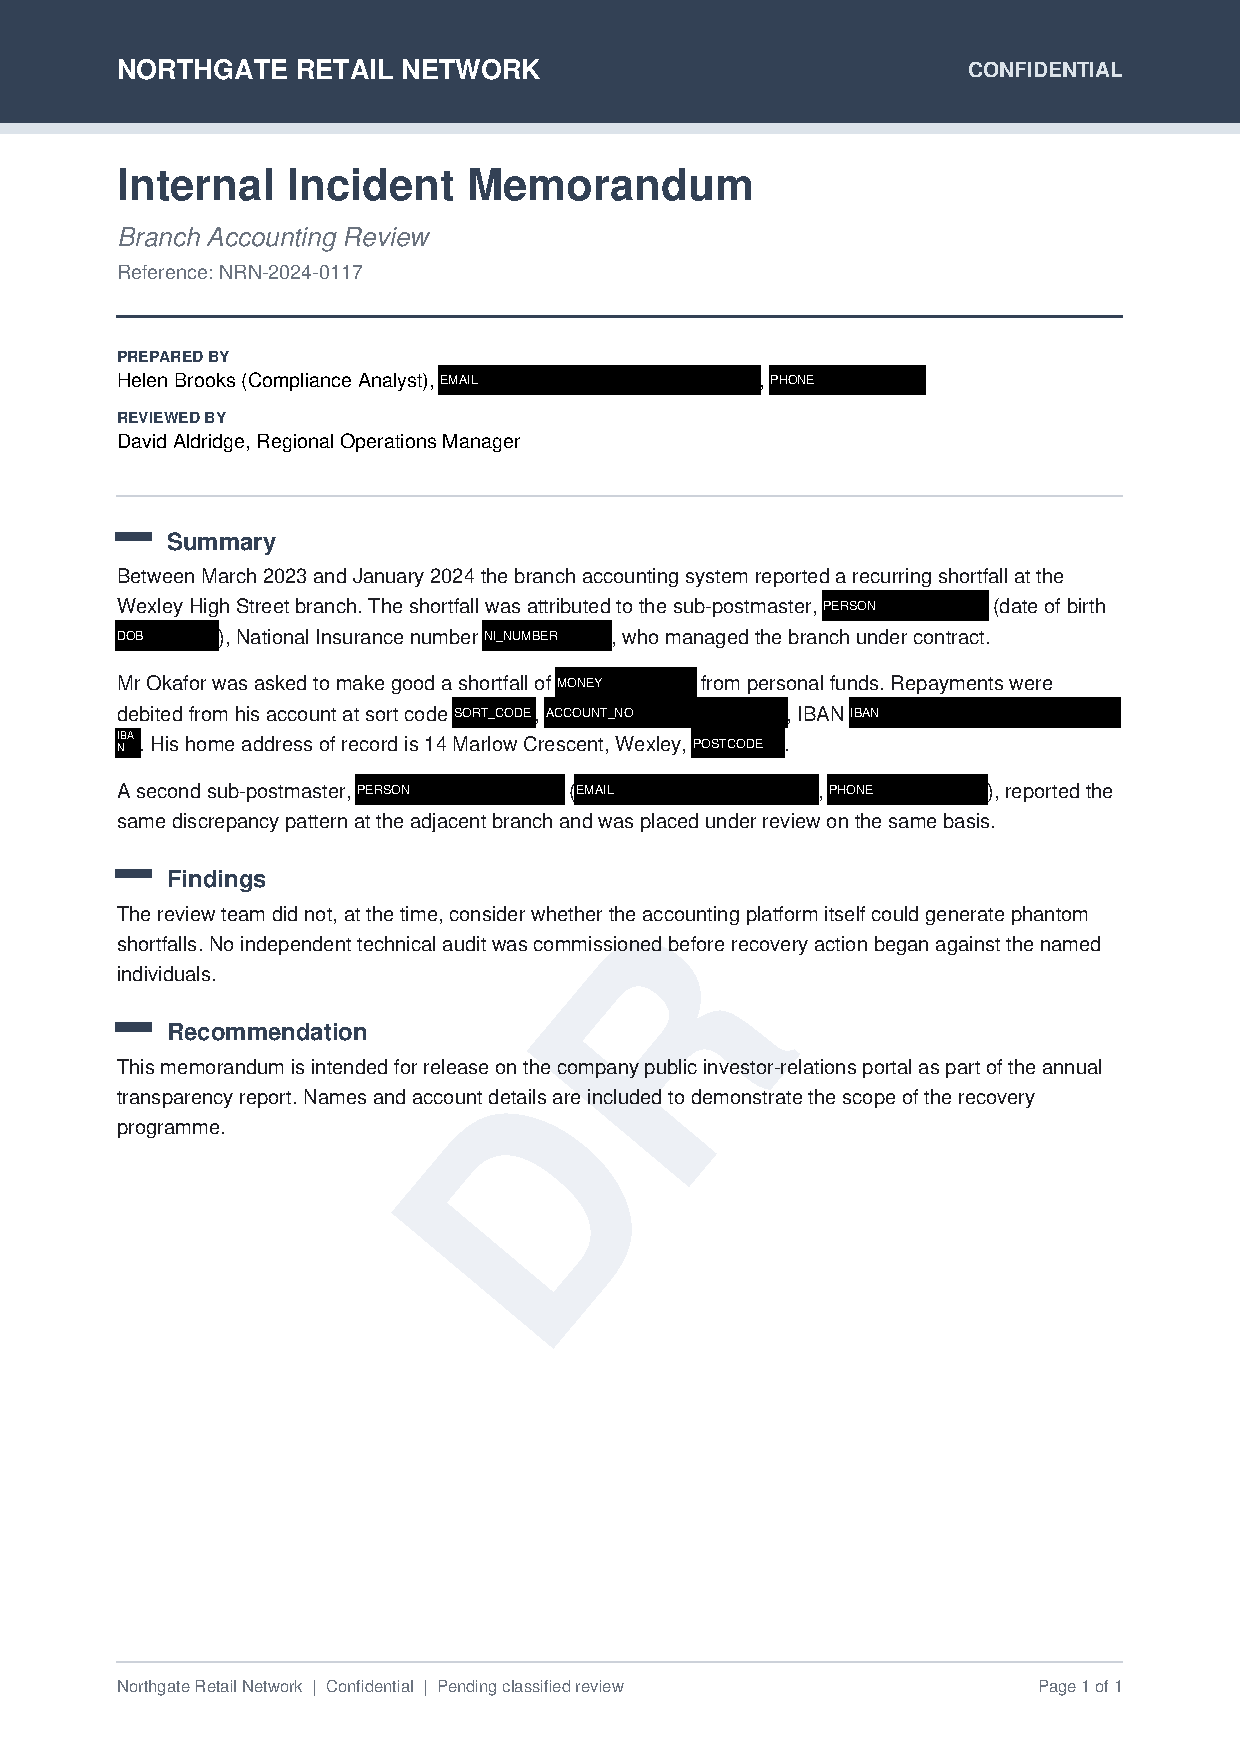
\includegraphics[width=0.78\textwidth]{redaction-demo/output/redacted_document.pdf}}
\caption{Prototype output: every detected item is replaced by a black bar tagged with its category. The narrative text (the absence of a technical audit before recovery) is preserved, so the document stays useful while the personal and financial data are removed.}
\label{fig:redacted}
\end{figure}

\subsection{Strengths and limitations}

The prototype is a faithful but deliberately minimal slice of the framework. Table~\ref{tab:prototype} states what it demonstrates and what it does not.

\begin{table}[H]
\centering
\small
\rowcolors{2}{accentlight!30!white}{white}
\begin{tabular}{@{} p{6.7cm} p{7.3cm} @{}}
\toprule
\textbf{\color{accentdark}What it demonstrates} & \textbf{\color{accentdark}What it does not (and why it is acceptable)} \\
\midrule
True redaction: the data leaves the file, verified by re-extraction & A regex detector misses untitled names (for example a name with no Mr/Mrs prefix); it is a stand-in for the GenAI proposer \\
Risk scoring and tiering drive the mandated human control automatically & No live LLM is called; detection is rule-based, so recall is partial by design \\
A hash-chained, append-only audit record with the paper's four field groups & The miss is the point: it makes the automation-bias argument concrete, the human reviewer must catch what the tool leaves (Section~\ref{sec:hitl}) \\
Publication stays blocked with no reviewer and no token, enforcing the gate & Single document, single page; it illustrates the control, it is not a production service \\
\bottomrule
\end{tabular}
\caption{Prototype scope: the controls it proves operate, and the boundaries it does not cross.}
\label{tab:prototype}
\end{table}

The negative result is as instructive as the positive one: detection is an aid to a human gate, not a replacement for it.

\newpage
% ============================================================
% REFERENCES
% ============================================================
\begin{thebibliography}{9}

\bibitem{falchi_slides}
Alessio Falchi.
\textit{Project \& Business Management: Course Slides}.
University of Pisa, 2024.

\bibitem{gdpr}
European Union.
\textit{General Data Protection Regulation (GDPR), Articles 5, 25 and 32}.

\bibitem{nist_ai_rmf}
National Institute of Standards and Technology.
\textit{Artificial Intelligence Risk Management Framework (AI RMF 1.0)}.
2023.

\bibitem{iso42001}
International Organization for Standardization.
\textit{ISO/IEC 42001:2023, Artificial Intelligence Management Systems}.
2023.

\bibitem{iso27001}
International Organization for Standardization.
\textit{ISO/IEC 27001:2022, Information Security Management Systems}.
2022.

\bibitem{ico2025}
Information Commissioner's Office.
\textit{Post Office Limited Reprimand}.
2025.

\bibitem{guardian2024}
The Guardian.
\textit{Post Office accidentally leaks names and addresses of wrongfully convicted operators}.
2024.

\end{thebibliography}

\end{document}
